\documentclass[12pt]{article}
\usepackage{xeCJK}%preamble part
\usepackage{graphicx}
\usepackage{indentfirst}
\usepackage[a4paper, inner=1.5cm, outer=3cm, top=2cm, bottom=3cm, bindingoffset=1cm]{geometry}
\usepackage{epstopdf}
\usepackage{listings}
\usepackage{array}
\usepackage{fontspec}
\usepackage{gensymb}
\usepackage{todonotes}
\usepackage{amsmath}
\usepackage[citecolor=blue]{hyperref}
\usepackage{makecell}
\usepackage[lofdepth,lotdepth]{subfig}




\setlength{\extrarowheight}{4pt}
\setlength{\parindent}{1cm}
\begin{document}
\title{\textbf{\fontsize{15.75pt}{\baselineskip}{讨论}}} 

\author{\fontsize{12pt}{\baselineskip}{数33 赵丰}}
\maketitle
\large
在协作定位中,假设其中一个移动节点是目标节点,能够与目标节点直接通信的移动节点属于第一层的节点$V_1$,能够与第一层的节点直接通信的节点属于第二层的节点,以此类推。我们按这种节点分层的顺序对$N_a$个移动节点重新编号,target agent为$v_1$,接下来是第一层的节点...
然后原来的FIM是一个三对角矩阵(每个矩阵的element都是2乘2的小矩阵),其他部分都是零元是因为由于距离和信噪比等原因两个节点无法直接通信而不产生信息。
由于沈老师的文献中已经指出了每个被定位的节点的FIM(2乘2)都可以写成$\sigma \lambda pp^T$,这里$Sigma$是对被定位节点和所有其他节点通信产生的信息的求和。这个式子可以拆成锚点和被定位节点的部分$\Sigma_i$与
所有其他移动节点和被定位节点的部分。对于后者,可以写成两个“向量”的內积,这里最小的element都是2乘2的小矩阵。
由于每一层的节点可能有多个,因此在你的论文中(比如定理2.3中)实际上每个小矩阵并不是2乘2的。但以下为了讨论方便,假设每一层只有一个节点,那么由沈老师给的全体移动节点的$2*N_a$维的FIM的表达式
$J_e(P,K)$可以很容易的化为下面的
形式:
\[
\left(
\begin{array}{ccccc}
\Sigma_0+B_0 B_0^H & -B_0 F_1^H & 0 &...& 0 \\
-F_1B_0^H & \Sigma_1+B_1 B_1^H +F_1 F_1^H & -B_1F_2^H & ...&0 \\
0&-F_2B_1^H&\Sigma_2+B_2B_2^H+F_2F_2^H & ...&0\\
&&...&&\\
0&...&0&-F_{K}B_{K-1}^H&\Sigma_K+F_K F_K^H
\end{array}
\right)
\]\newpage
上式和你的论文中的定理2.3中的最后一行不一样,个人觉得定理2.3可能有笔误,理由如下:
$B_i$中的B表示backward,F表示forward,如下图所示
\begin{figure}[!ht]
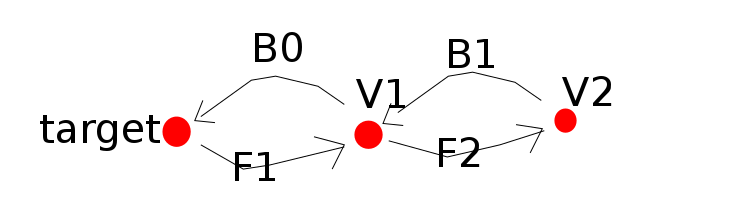
\includegraphics[width=\linewidth]{001.png}
\end{figure}

在只有一个目标节点$V_0$时,定位信息只能依靠它和锚点的通信得到,此时
$J_e(P,0)=\Sigma_0$.当有两个移动节点时,目标节点的定位信息增加了
来自V1的后向信息B0,而V1的定位既有来自锚点的定位信息$\Sigma_1$,又有来自V0的前向信息F1,因此
\[
J_e(P,2)=\left(
\begin{array}{cc}
\Sigma_0+B_0 B_0^H & -B_0 F_1^H\\
-F_1 B_0^H & \Sigma_1+F_1 F_1^H
\end{array}
\right)
\]
注意到在只有两个移动节点的情况下,没有B1的贡献,由上图也可以看出,B1是第三个移动节点(第二层)的后向信息。因此定理2.3对于k=1
不成立。
在按照上面给出的$J_e(P,k)$的表达式后,定理2.4给出了计算某一层的网络节点对参与协作的贡献。由于$J_e(P,k)$是三对角的稀疏矩阵,因此
由定义2.6应该可以进一步化简出$J(k)$的表达式。
你考虑的可能是每个小矩阵由于每层节点数大于1不是2乘2的,但在分块矩阵的运算过程中,小矩阵的具体大小不影响基本运算,为了方便讨论和证明,以下仍默认所有的小矩阵都是2乘2的。
定义2.6应改为$J(k)=tr(J^{-1}_e(P,k-1)-J^{-1}_e(P,k))$
你给的证明可能是我不理解符号体系,我看不太懂,我仿照你的思路推导定理2.4给出的J(k)表达式,我只推导出J(1)的表达式,附录中从k到k+1的归纳我不明白为什么J(k+1)直接就具有那样的形式?
以下为简便,取trace的符号省略不写:
(注:这个结论用Woodbury矩阵求逆公式很快变可以推出)
\begin{equation}\label{eq:S1}
J(1)=\Sigma_0^{-1} B_0 (I+B_0^H \Sigma_0^{-1} B_0+F_1^H \Sigma_1^{-1} F_1 )^{-1} B_0^H \Sigma_0^{-1}
\end{equation}•
$J_e^{-1}(P,0)=\Sigma_0^{-1}$
由EFIM可知,
\[
J_e^{-1}(P,1)=(\Sigma_0+B_0B_0^H-B_0F_1^H(\Sigma_1+F_1F_1^H)^{-1}F_1B_0^H)^{-1}
\]
\[
=(\Sigma_0+B_0B_0^H-B_0(F_1^{-1}\Sigma_1F_1^{-H}+I)^{-1}B_0^H)^{-1}
\]
\[
J_e^{-1}(P,0)-J_e^{-1}(P,1)
=\Sigma_0^{-1}-(\Sigma_0+B_0B_0^H-B_0(F_1^{-1}\Sigma_1F_1^{-H}+I)^{-1}B_0^H)^{-1}
\]
\[
=(\Sigma_0^{-1}(\Sigma_0+B_0B_0^H-B_0(F_1^{-1}\Sigma_1F_1^{-H}+I)^{-1}B_0^H)-I)
\]
\[
(\Sigma_0+B_0B_0^H-B_0(F_1^{-1}\Sigma_1F_1^{-H}+I)^{-1}B_0^H)^{-1}
\]
\[
=(\Sigma_0^{-1}(B_0B_0^H-B_0(F_1^{-1}\Sigma_1F_1^{-H}+I)^{-1}B_0^H))(\Sigma_0+B_0B_0^H-B_0(F_1^{-1}\Sigma_1F_1^{-H}+I)^{-1}B_0^H)^{-1}
\]
\[
=(\Sigma_0^{-1}(B_0(F_1^{-1}\Sigma_1F_1^{-H}+I-I)(F_1^{-1}\Sigma_1F_1^{-H}+I)^{-1}B_0^H))
\]
\[
(\Sigma_0+B_0B_0^H-B_0(F_1^{-1}\Sigma_1F_1^{-H}+I)^{-1}B_0^H)^{-1}
\]
\[
=(\Sigma_0^{-1}(B_0F_1^{-1}\Sigma_1F_1^{-H}(F_1^{-1}\Sigma_1F_1^{-H}+I)^{-1}B_0^H))(\Sigma_0+B_0B_0^H-B_0(F_1^{-1}\Sigma_1F_1^{-H}+I)^{-1}B_0^H)^{-1}
\]
\[
=(\Sigma_0^{-1}B_0(B_0^{-H}(F_1^H\Sigma_1^{-1}F_1+I))^{-1})(\Sigma_0+B_0B_0^H-B_0(F_1^{-1}\Sigma_1F_1^{-H}+I)^{-1}B_0^H)^{-1}
\]
\[
=\Sigma_0^{-1}B_0((\Sigma_0+B_0B_0^H-B_0(F_1^{-1}\Sigma_1F_1^{-H}+I)^{-1}B_0^H) (B_0^{-H}(F_1^H\Sigma_1^{-1}F_1+I)))^{-1}
\]
\[
=\Sigma_0^{-1}B_0(\Sigma_0 B_0^{-H}(F_1^H\Sigma_1^{-1}F_1+I)+B_0(F_1^H\Sigma_1^{-1}F_1+I)-B_0
\]
\[
(F_1^{-1}\Sigma_1F_1^{-H}+I)^{-1}(F_1^H\Sigma_1^{-1}F_1+I))^{-1}
\]
\[
=\Sigma_0^{-1}B_0(\Sigma_0 B_0^{-H}(F_1^H\Sigma_1^{-1}F_1+I)+B_0(F_1^H\Sigma_1^{-1}F_1+I)-B_0F_1^H\Sigma_1^{-1}F_1)^{-1}
\]
\[
=\Sigma_0^{-1}B_0(\Sigma_0 B_0^{-H}(F_1^H\Sigma_1^{-1}F_1+I)+B_0)^{-1}
\]
上式进一步化简可得(\ref{eq:S1})

\end{document}